\section{Discussion}

\begin{figure}
\centering
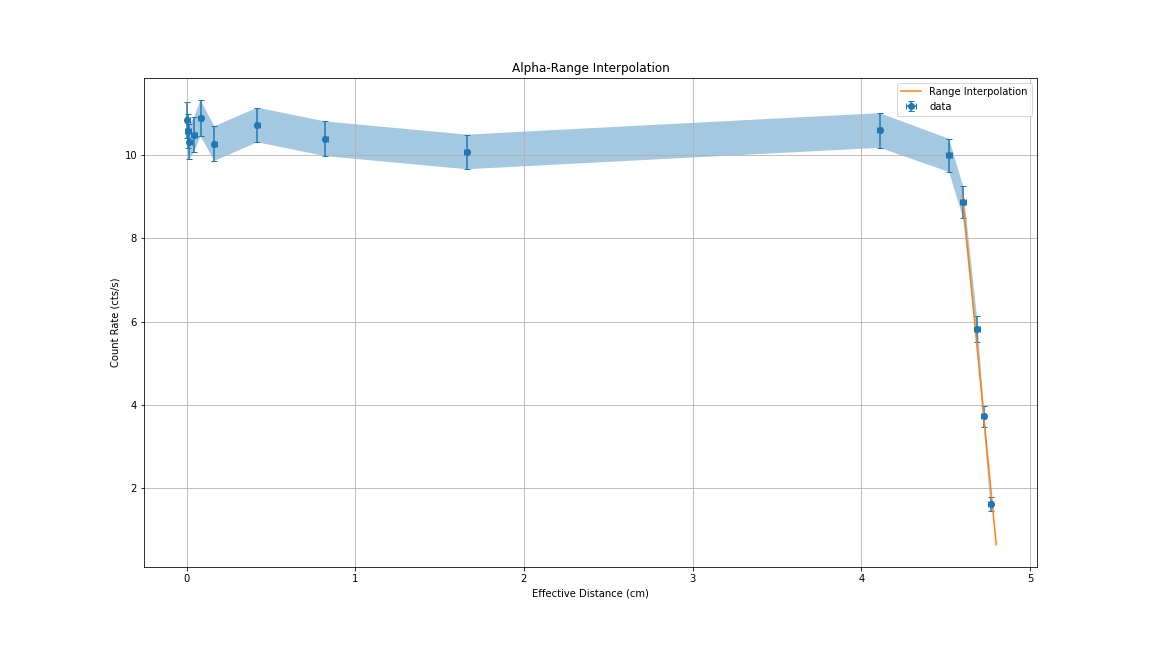
\includegraphics[width=\textwidth]{count_rate.png}
\caption{The detector count rate of the $\alpha$ energy peak as a function of effective distance. This shows that after some amount of absorbing material, $\alpha$ particles are not able to continue travelling and are stopped/absorbed. The end of this distribution can be interpreted as the range of $\alpha$ particles in this medium at the characteristic energy. It can be measured by interpolating the linear portion of the distribution and extrapolating that value to a count rate of 0.}
\label{fig:count-rate}
\end{figure}

The peak position, in terms of energy/channel number, as a function of pressure (or proportionally effective distance) certainly changes with pressure. There is a very strict decrease in peak position as pressure increases as seen in Fig. \ref{fig:peak-position}. The peak width as a function of pressure has a less clear relationship. As pressure increases, it seems at first to proportionally increase the peak width. But at high pressures this is less clear, as there is significant variation in peak width for relatively close pressure values. This would indicate that while the position of the peak depends on pressure, there is no clear dependence of the peak width on pressure. The peak position’s relationship with pressure can be explained by the scattering behavior of the $\alpha$ particles being detected. At lower pressures, there is very little absorbing medium to reduce the full energy of the $\alpha$ particle, so its full energy is deposited in the detector. At higher pressures, the medium scatters the $\alpha$ particle more and thus the energy deposited is less, and then the channel of the peak in the MCA is smaller.

\begin{figure}
\centering
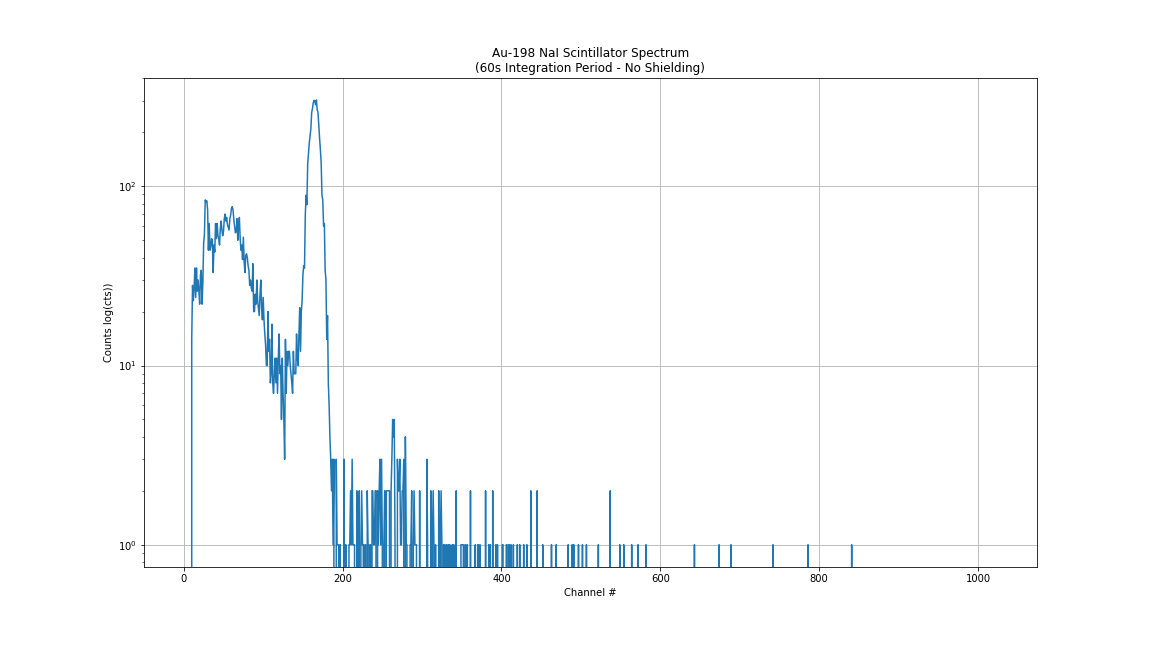
\includegraphics[width=\textwidth]{au198_spectrum.png}
\caption{Representative ${}^{198}Au$ energy spectrum plotted in a semi-logarithmic (y) scale. While this spectrum has not been energy calibrated, the 411.8 keV photopeak is clearly visible and intense enough to record peak statistics.}
\label{fig:au198-spectrum}
\end{figure}

The mean stopping power has a delayed response to changes in the mean energy in that it has slower growth for a range of several MeV and then exponentially rises when some threshold is met. The opposite is true for mean stopping power as a function of effective distance, where the stopping power is larger and larger as the effective distance reaches zero, but is relatively constant, near zero, for longer effective distances. The behavior of the mean stopping power regarding mean energy is most likely due to less power being required to stop lower energy particles compared to higher energy particles. As the mean energy of the $\alpha$ particle reaches its maximum energy (5.486 MeV), the mean stopping power exponentially asymptotes to infinity. This means that a higher energy particle will lose more energy per unit length since it has more to shed before being stopped. Mean stopping power is relatively flat for effective distances farther away from zero. This behavior is indicative of the fact that the lower effective distances mean less medium is required to stop the particle. That means that the stopping power will be higher since significantly more energy is lost per unit length compared to a longer effective distance for the same energy particle.

\begin{figure}
\centering
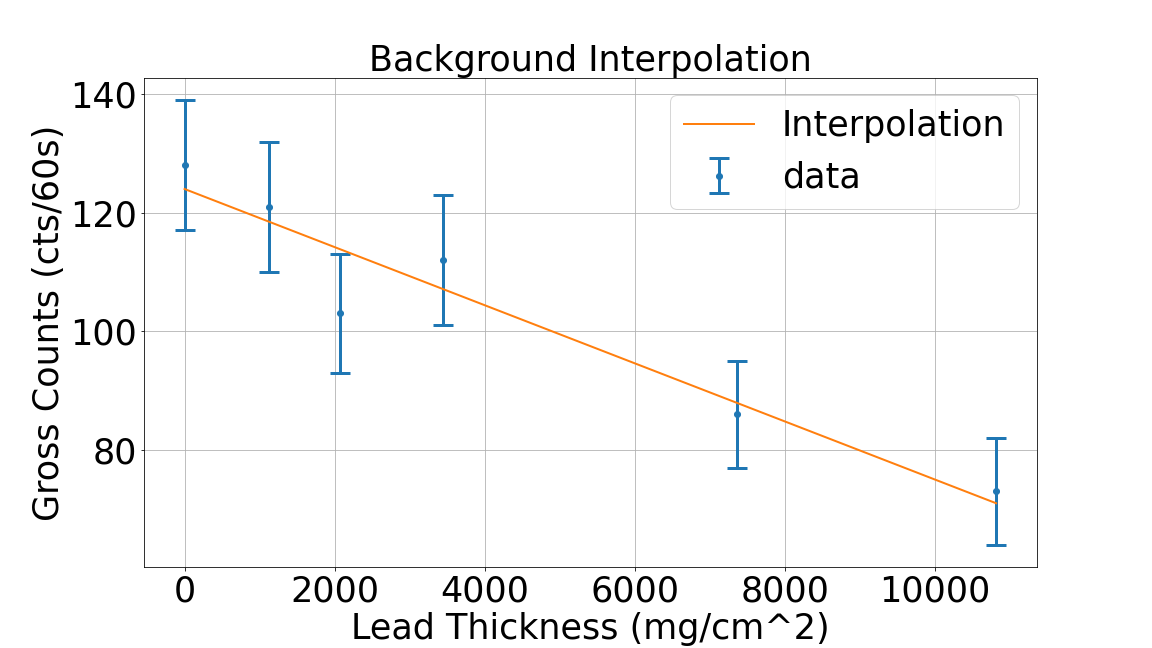
\includegraphics[width=\textwidth]{background.png}
\caption{The background radiation detected in the NaI scintillator is plotted here. This data is collected by recording measurements at varying lead shielding thickness with the radiation source plugged. The background is assumed to be linear in regard to the shielding thickness and a linear relationship is plotted and interpolated.}
\label{fig:background}
\end{figure}

\begin{figure}
\centering
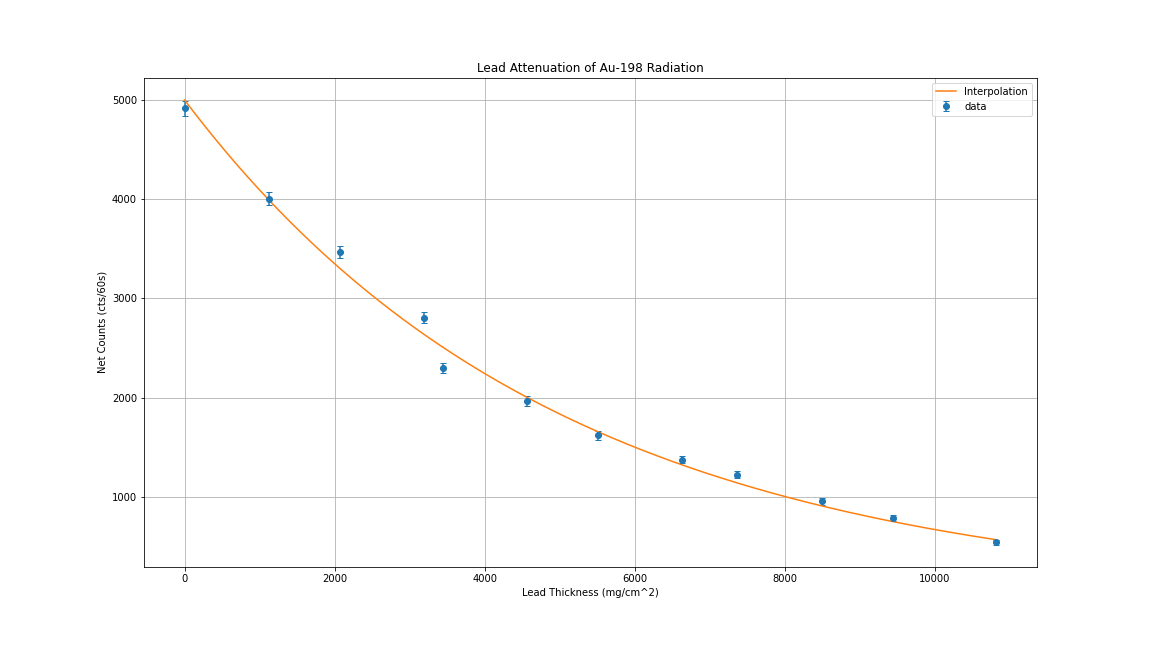
\includegraphics[width=\textwidth]{Pb.png}
\caption{The attenuation of gamma radiation is plotted for different thicknesses of lead. The data exhibits an exponential decay behavior indicative of gamma attenuation. This data can be fitted to a characteristic function and the mass attenuation coefficient can be extracted from the fit.}
\label{fig:Pb}
\end{figure}

\begin{figure}
\centering
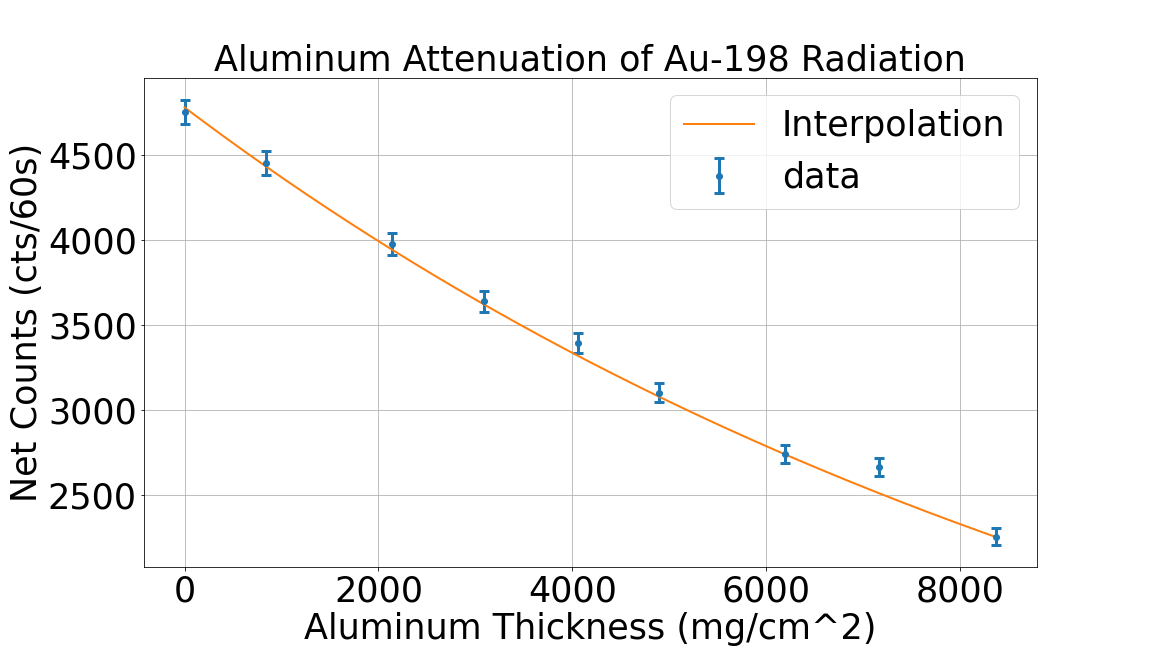
\includegraphics[width=\textwidth]{Al.png}
\caption{The attenuation of gamma radiation is plotted for different thicknesses of aluminum. The data exhibits an exponential decay behavior indicative of gamma attenuation. This data can be fitted to a characteristic function and the mass attenuation coefficient can be extracted from the fit.}
\label{fig:Al}
\end{figure}

The range for $\alpha$ particles extracted above was $R_{\alpha}$ = 4.81 $\pm$ 0.43 cm. The expected range value for an alpha particle with energy ~5.5 MeV in air is about 4.12 cm \cite{nistrange}. That means the range calculated in this work is slightly larger than expected and just beyond uncertainty of the expected value. It is unsurprising that the range presented is larger than the expected because of the nature of its calculation. This range was extrapolated using a linear approximation of the end of the count-rate distribution. Since the linear interpolation was propagated to zero count-rate, this range value will be at the very end of the distribution. The range is actually defined as the mean of the linear region in the count-rate distribution \cite{knoll}. Thus, the actual range is expected to be larger than a linear extrapolation like this one.

A collimated source is preferable for measuring gamma attenuation because it prevents discrepancy in measurement due to several physical phenomena. When the source is collimated, attenuation due to material is incident on the material. If this was not the case, the measurement of the attenuation coefficient would maintain uncertainty associated with “glancing” collisions between the radiation and the shielding material. These interactions occur on an angle and thus do not reflect the full attenuating power of the shielding material.

Expected mass attenuation coefficients are collected from NIST \cite{nist}. The expected value for lead is approximately 2.323 $\times 10^{-4}$ $(\frac{mg}{cm^2})^{-1}$ and for aluminum is 9.276 $\times 10^{-5}$ $(\frac{mg}{cm^2})^{-1}$ when the $\gamma$ radiation detected is approximately at the ${}^{198}Au$ photopeak of 411.8 keV. The results for lead reported in this work is very close to the expected value but within a few uncertainties of it, likewise for the reported aluminum mass attenuation coefficient. Several explanations can provide for the difference. For one, the mass attenuation coefficient depends on the energy of the radiation being shielding. This experiment utilizes the 411.8 keV photopeak produced by ${}^{198}Au$. Association is made by comparing the net counts of the 411.8 keV photopeak at each thickness of shielding material. However, uncertainties exist relating to the measurement of this net count. The net count is calculated using a linear interpolation of the background and subtracting this from the gross counts measured by the data acquisition software. The linear interpolation is an imperfect solution to measuring the background radiation, as uncertainties exist for the interpolation at each thickness. In addition to this, the software has uncertainties associated with the measurement of the gross counts. It should also be noted that the expected value reported from NIST is given for $\gamma$ radiation at an energy of 400 keV, not 411.8 keV. Since mass attenuation coefficients are only reported at intervals, this was as close as could be found. All these uncertainties compound when calculating the mass attenuation coefficient and can ultimately lead to discrepancies in the result.

In review, values reported for the $\alpha$ particle range and mass attenuation coefficients for lead and aluminum are acceptable reproductions of expected values when discrepancies are explained. This completes a review of two very important and common measurements of radiation deposition. With this knowledge, safety designs can be implemented that protect against radiation with these particular specifications.
